\documentclass{article}

\usepackage[margin=1.2in]{geometry}
\usepackage{graphicx}
\usepackage{amsmath,amssymb,amsthm,bm}
\usepackage{latexsym,color,minipage-marginpar,caption,multirow,verbatim}
\usepackage{enumerate}
\usepackage[round]{natbib}
\usepackage{times}
\usepackage{booktabs}
\usepackage{array}
\usepackage{parskip}
\usepackage{float}

\newcommand{\cP}{\mathcal{P}}
\newcommand{\cX}{\mathcal{X}}
\newcommand{\cR}{\mathcal{R}}
\newcommand{\cT}{\mathcal{T}}
\newcommand{\cY}{\mathcal{Y}}
\newcommand{\cQ}{\mathcal{Q}}

\newcommand{\EE}{\mathbb{E}}
\newcommand{\PP}{\mathbb{P}}
\newcommand{\QQ}{\mathbb{Q}}
\newcommand{\RR}{\mathbb{R}}
\newcommand{\ZZ}{\mathbb{Z}}

\newcommand{\Var}{\textnormal{Var}}
\newcommand{\Cov}{\textnormal{Cov}}
\newcommand{\MSE}{\textnormal{MSE}}
\newcommand{\toProb}{\overset{p}{\to}}
\newcommand{\toPtheta}{\overset{{P_\theta}}{\to}}

\newcommand{\union}{\cup}
\newcommand{\intersect}{\cap}
\newcommand{\RIGHT}{\Longrightarrow}
\newcommand{\LEFT}{\Longleftarrow}
\newcommand{\IFF}{\Longleftrightarrow}
\newcommand{\es}{\varnothing}

\newcommand{\indicator}[1]{\mathbf {1} _{#1}}
\newcommand{\h}[1]{\hat{#1}}
\newcommand{\lbar}[1]{\overline{#1}}

\newcommand{\pref}{\succsim}
\newcommand{\spref}{\succ}





\DeclareMathOperator*{\argmax}{argmax}
\DeclareMathOperator*{\argmin}{argmin}


\newcommand{\simiid}{\overset{\text{i.i.d.}}{\sim}}
\newcommand{\simind}{\overset{\text{ind.}}{\sim}}
\newcommand{\ep}{\varepsilon}

\newcommand{\bhat}{\hat{\beta}}
\newcommand{\btil}{\tilde{\beta}}
\newcommand{\ehat}{\hat{e}}
\newcommand{\etil}{\tilde{e}}
\newcommand{\Yhat}{\hat{Y}}
\newcommand{\Ybar}{\overline{Y}}
\newcommand{\tr}{\operatorname{tr}}
\newcommand{\m}[1]{\begin{bmatrix}
#1
\end{bmatrix}}

\definecolor{darkblue}{rgb}{0.2, 0.2, 0.5}

\newenvironment{solution}{~\\\color{darkblue}{\bf Solution:~\\}}{}
\newenvironment{ifsol}{\color{darkblue}}{}

\newcommand{\optional}{{\bf Optional:} (Not graded, no extra points) }
\newcommand{\tn}[1]{\textnormal{#1}}

\graphicspath{{../output/}{output/}}
\newcommand{\outfig}[3][0.7]{%
  \begin{figure}[htbp]
    \centering
    \includegraphics[width=#1\textwidth]{#2}
    \caption{#3}
    \label{fig:#2}
  \end{figure}}

\theoremstyle{definition}
\newtheorem{problem}{Problem}
\title{ECON 109 Election Prediction Write-Up: Ohio Senate
  }
\date{}
\begin{document}
\maketitle

\section*{Introduction}
The subject of this report is the 2026 special election for Ohio's Class 3 Senate seat. JD Vance won this seat in 2022 with a two party vote share of 53\% against the Democratic nominee, Tim Ryan. When the Trump-Vance ticket won the 2024 presidential election, Vance vacated the seat, and Ohio's governor, Mike DeWine, appointed his lieutenant governor, Jon Husted, to fill it. Husted is also the Republican nominee in the special election.

The Democratic nominee is Sherrod Brown. Brown held Ohio's Class 1 Senate seat from 2007 until 2025, but he lost it to Bernie Moreno in 2024 with a two party vote share of 48.1\%. However, he ran about 4 percentage points ahead of Kamala Harris, whose two party vote share in Ohio was 44.3\%.

\outfig[0.6]{ohio_statewide_races}{Democratic two party margin in Ohio statewide races, 2000--2024.}

Figure~\ref{fig:ohio_statewide_races} plots every statewide race in Ohio since 2000. The Democratic win in the 2006 governor's race is an outlier. Scandals surrounding the outgoing Republican governor, Bob Taft, made the Republican nominee, Ken Blackwell, deeply unpopular in a year that already favored Democrats nationally. From 2000 to 2012, Ohio's Democratic two party presidential margin stayed close to zero, and the state was a bellwether for every presidential election in that period. Brown's 2006 win came with the Democratic wave in the midterm after Bush's 2004 re-election. He won re-election in 2012, running ahead of Obama, and again in 2018, while Republicans won every governor's race after 2006: John Kasich in 2010 and 2014, and Mike DeWine in 2018 and 2022. Husted was DeWine's running mate in both of DeWine's wins, and their large margin in 2022 also reflects the midterm backlash against the Democratic president elected in 2020. Husted was also elected Ohio Secretary of State in 2010 and 2014, with two party vote shares of 56.8\% and 62.7\%.

To conclude, Sherrod Brown, a popular former senator, faces Jon Husted, a well-known figure who has not faced Ohio's voters on his own since 2014, as his two statewide wins since then came on Mike DeWine's ticket.

\section*{Baseline}

The baseline model estimates the following equation:
\[S_{s,t} = b_0 + b_1 L_{s, \tau (t)} + b_2\text{MidD}_t + b_3\text{MidR}_t + b_4 S_{s,\rho(t)} + u_{s, t}.\]
While $s$ and $t$ are used as subcripts, a state that held a regular and a special election in the same year contributes two observations, so their usage is more conceptual than for the purpose of indexing observations. Tables $1$ and $2$ define variables and reports the OLS results. 

\begin{table}[!htbp]
  \centering
  \scriptsize
  \renewcommand{\arraystretch}{1.05}
  \caption{Variable definitions}
  \label{tab:vars}
  \setlength{\tabcolsep}{4pt}
  \begin{tabular}{l >{\raggedright\arraybackslash}p{7.6cm} >{\raggedright\arraybackslash}p{4.5cm}}
    \toprule
    Notation & Description & Source \\
    \midrule
    $s$, $t$ & State, and election year (an even year from 2000 to 2024, midterm or presidential). & Included with data \\
     $\tau(t)$ & The last presidential election before year $t$ (2024 for 2026). & Constructed \\
     $\rho(t)$ & The year of state $s$'s most recent Senate race before $t$ (2024 for Ohio in 2026). & Constructed  \\
    $S_{s,t}$ & Democratic two party vote share in state $s$'s Senate race in year $t$, in percent. & MIT Election Data and Science Lab \\
    $P_{s,t}$, $P_{\text{US},t}$ & Democratic two party vote share for president in state $s$, and nationally, in presidential year $t$. & MIT Election Data and Science Lab\\
    $L_{s,\tau(t)}$ & $P_{s,\tau(t)} - P_{US,\tau(t)}$ & Constructed from $P_{s,t}$ and $P_{\text{US},t}$ \\
    $\text{MidD}_t$, $\text{MidR}_t$ & Dummies for $t$ being a midterm year with a Democratic president and one a Republican president, respectively & Constructed from the sitting president's party \\
    $u_{s,t}$ & The part of $S_{s,t}$ that the other variables do not explain. & Inherently unknown, but estimated with OLS \\
    \bottomrule
  \end{tabular}
\end{table}

Each $b_i$ is estimated by OLS, and the standard errors are clustered by state. This means that we assume $\Cov(u_{s,t}, u_{s',t'}) = 0$ for $s \neq s'$, while $u_{s,t}$ and $u_{s,t'}$ can be correlated across different years within the same state. Persistent state-specific factors, such as the strength of a state's party organizations, are therefore accounted for in the standard errors. National shocks that affect every race in a given year, such as an oil shock or the Great Recession, are not, so the standard errors on $\text{MidD}_t$ and $\text{MidR}_t$, which vary only by year, are likely too small.



\begin{table}[!htbp]
  \centering
  \footnotesize
  \setlength{\tabcolsep}{4pt}
  \caption{Baseline regressions of the Democratic two party vote share in Senate races}
  \label{tab:baseline}
  \begin{tabular}{l*{3}{c}}
    \toprule
    & \multicolumn{3}{c}{Dependent variable: $S_{s,t}$} \\
    \cmidrule(lr){2-4}
    & (1) & (2) & (3) \\
    \midrule
    Partisan lean, $L_{s,\tau(t)}$ & $0.991$ & $0.988$ & $0.846$ \\
     & $(0.056)$ & $(0.057)$ & $(0.125)$ \\[1pt]
    Midterm, Democratic president, $\text{MidD}_t$ &  & $-0.030$ & $-0.038$ \\
     &  & $(0.007)$ & $(0.007)$ \\[1pt]
    Midterm, Republican president, $\text{MidR}_t$ &  & $0.023$ & $0.024$ \\
     &  & $(0.010)$ & $(0.011)$ \\[1pt]
    Lagged Senate share, $S_{s,\rho(t)}$ &  &  & $0.145$ \\
     &  &  & $(0.096)$ \\[1pt]
    Constant & $0.520$ & $0.523$ & $0.453$ \\
     & $(0.007)$ & $(0.007)$ & $(0.051)$ \\[1pt]
    \midrule
    $R^2$ & 0.531 & 0.550 & 0.613 \\
    Races (observations) & 423 & 423 & 373 \\
    \midrule
    2026 Ohio baseline, Dem.\ margin & $-5.6$ & $-0.6$ & $+1.2$ \\
    \bottomrule
  \end{tabular}
\end{table}
Note that the last row is in terms of percentages while every figure (coefficient or standard error) is just a decimal value. 

The intuition for each variable should be somewhat clear. The Partisan lean variable roughly tracks how Democratic or Republican each state is, the midterm indicators cover the phenomenon of midterm backlash against the incumbent president's party, and the lagged Senate share is used since that's the only other bit of information we have about any particular state's Democratic senate performance. 

The results of the regression indicate that state-by-state partisanship and a constant term explain over half of the variation. Incoportating the midterm dummies marginally increase the $R^2$, but change the baseline margin prediction by about $5$ percentage points, which isn't unreasonable given that both coefficients are statistically significant. Adding lagged senate share does significantly increase the $R^2$, which shows that there is some difference in Senate \& Presidential race dynamics although it isn't at all clear which real world factors are driving that. 

The baseline prediction of a Democratic two party vote share margin of $1.2$ does seem reasonable given how narrowly Brown lost by and also the strength of the Republican nominee. But, given the size of the standard errors on the midterm dummies, lagged Senate share and the unexplained variation, this prediction should indicate that this is still a toss-up.  


\section*{Beyond the Baseline}
This model is of course not perfect, and has some other intuitive deficiencies. First off, there's no accounting of who is an incumbent and how much better they might perform past the first time they're elected. Beyond that, there is no consideration for candidate specific effects (in terms of policy positions or other characteristics), and both of these are specific to Ohio. Brown has done much better in the Senate than other Democrats who try to run for Ohio's other Senate seat. One could either chalk this up to the blue wave/midterm backlash in $2006$ and incumbency effects, but another contributing factor could be Brown's populism and relatively better appeal to non-college White voters. Additionally, a model incoporating these elements still wouldn't account for real-world dynamics and the strength of the Republican nominee, which recent polling information would provide an important disciplinary force.

This section will be devoted to dealing with these issues with particular statistics that come under the jurisdiction of the following subsections.

\subsection*{Campaign Finance}

Let's start off with campaign finance and restrict our attention to expenditures that are within the purview of the candidates, but still includes ads and whatnot. Looking at Figure 2, it is clear that Brown's campaign is spending much more on this race, which reflects how much they themselves raised by looking at Figure 1. 

\begin{figure}[H]
  \centering
  \begin{minipage}[t]{0.49\textwidth}
    \centering
    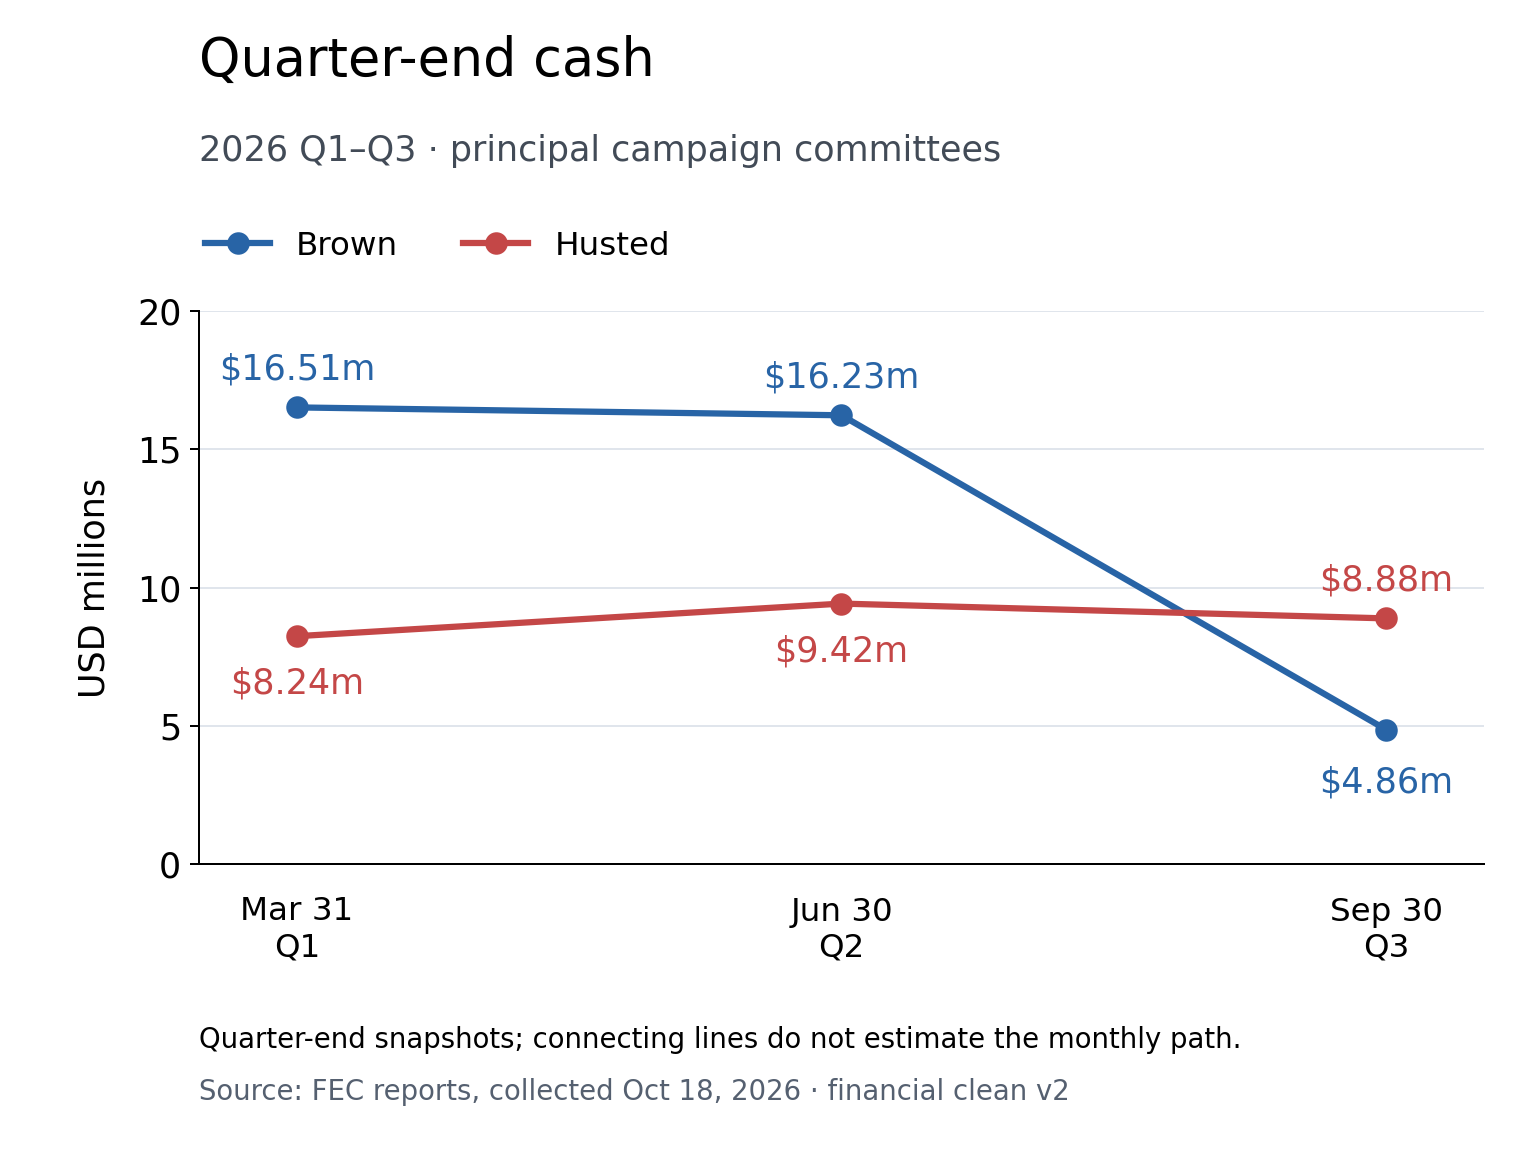
\includegraphics[width=\linewidth]{campaign_finance/cash_trend_2026_v1}
    \caption{Quarter-end cash on hand, 2026 Q1--Q3.}
    \label{fig:cf_cash}
  \end{minipage}\hfill
  \begin{minipage}[t]{0.49\textwidth}
    \centering
    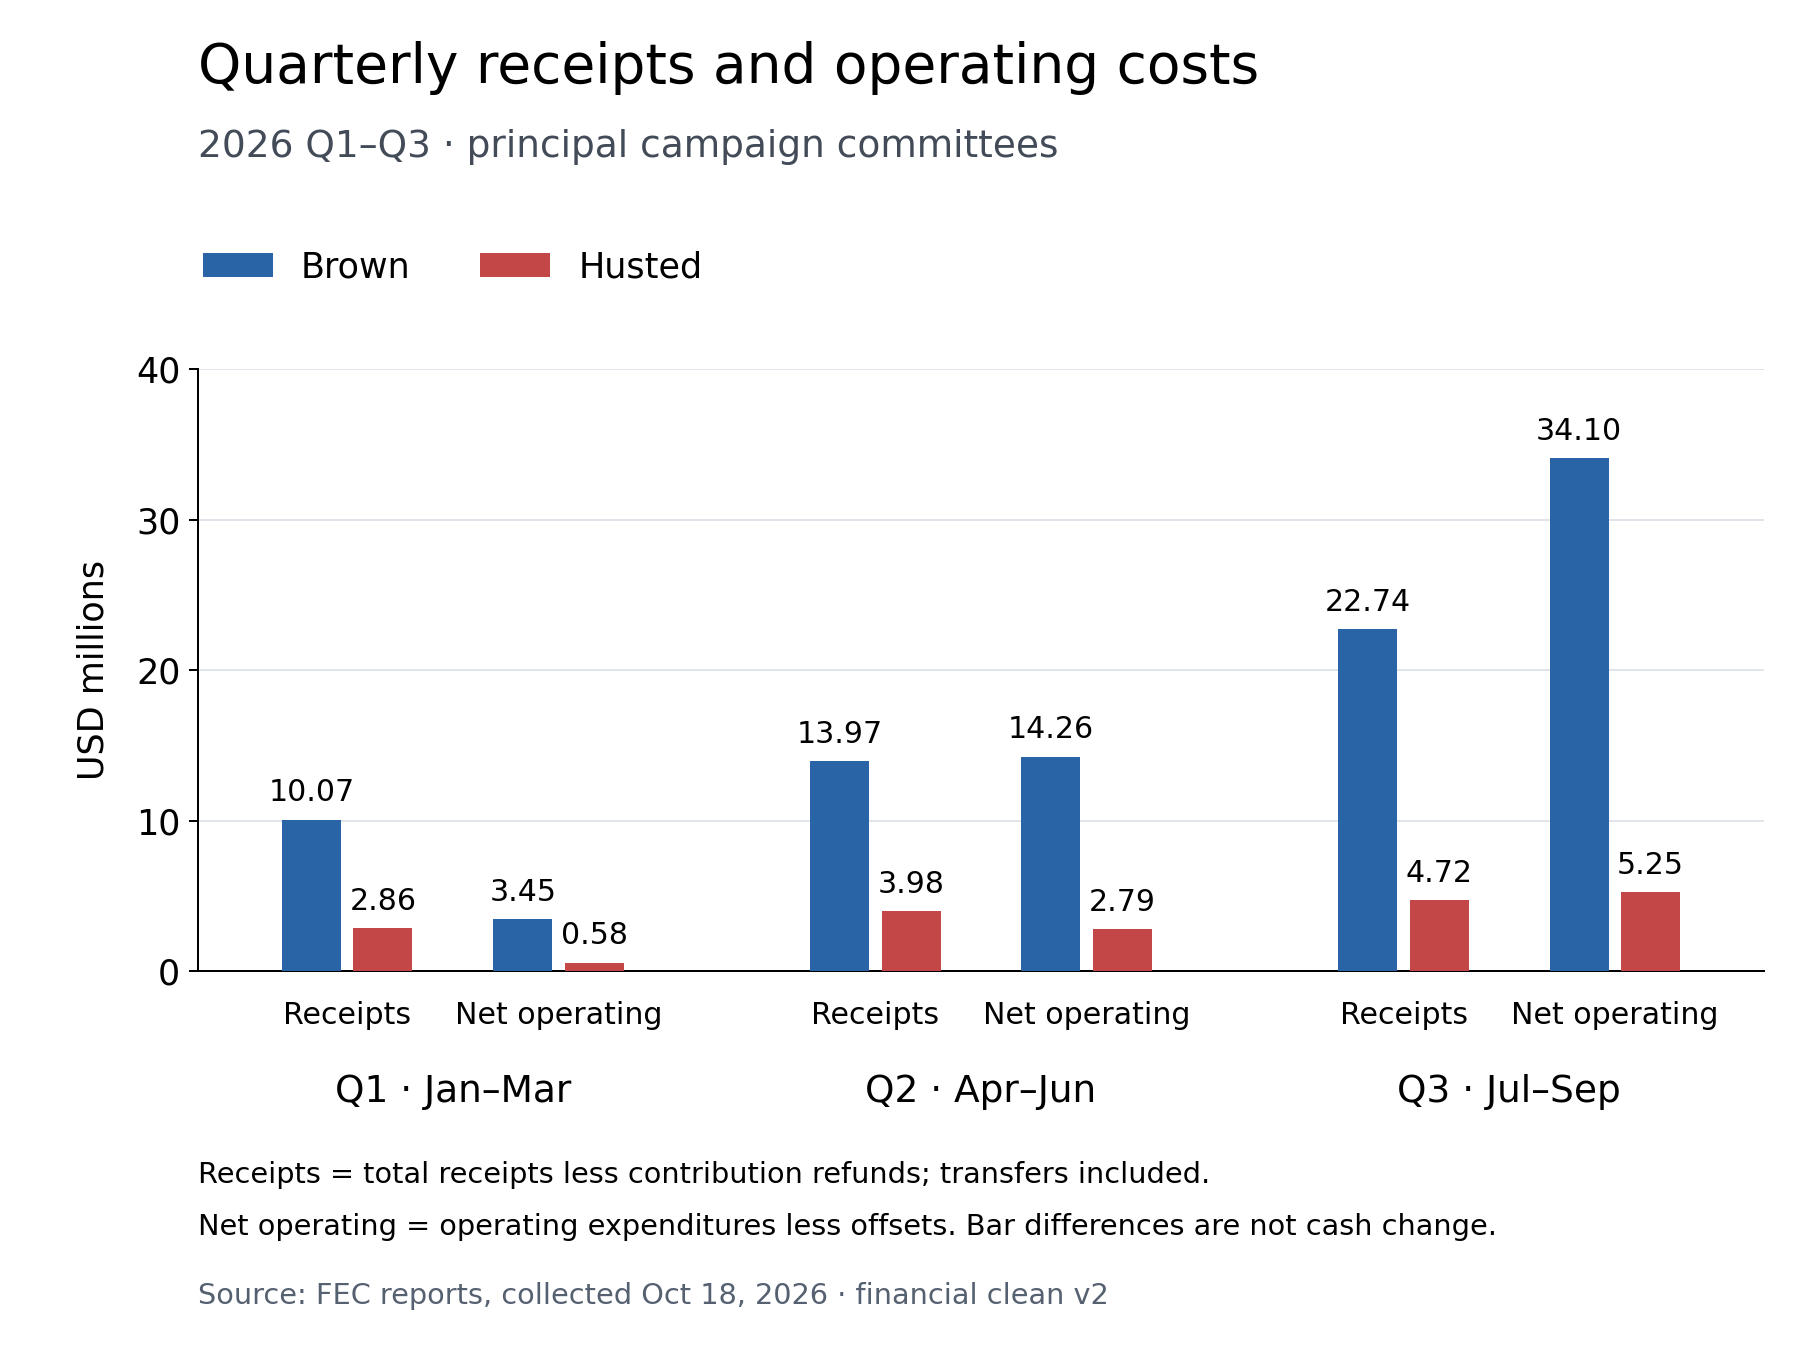
\includegraphics[width=\linewidth]{campaign_finance/quarterly_receipts_and_costs_v1}
    \caption{Quarterly receipts and net operating expenditures, 2026 Q1--Q3.}
    \label{fig:cf_quarterly}
  \end{minipage}
\end{figure}

Specifically, Brown raised 46.8 million versus Husted's 11.6 and outspent him (difference of receipts and net of operating costs figures) 51.8 million against 8.6 million. 

Our conclusion is that this is a very competitive race, and the spending amounts should reflect the relatively higher will among Democrats and Brown to reclaim another senate seat. Husted spending less than Brown shouldn't necessarily be taken as him running a weaker campaign, but confirms the idea that he does have name recognition and functions as an incumbent despite not being formally elected to senate. 

These figures will not formally go into our final model that will provide our prediction, but they serve to clarify the on-the-ground reality that this is a race that Democrats believe they can win despite the relatively strong Republican. 


\subsection*{Polling}

Five nonpartisan likely-voter polls fielded in the final three weeks of the campaign give Brown an average two party margin of $+4.7$. Given how these polls were selected, on recency (Oct 13 = 3 weeks before Nov 3rd), a likely-voter screen and nonpartisan sponsorship, we only consider their point estimates and disregard margin of error. Additionally, in 2022 and 2024, late Senate polling averages overstated Democrats by $2.4$ points on average, so subtracting that bias gives a poll-based estimate of Brown $+2.3$.

All relevant summary statistics are in the tables below and the timeseries plot gives an ideas of how, while this poll-based estimate does go toward Brown, the margin of error is greater than the margin since sampling variability is still quite high. 



\begin{figure}[H]
  \centering
  \begin{minipage}[c]{0.56\textwidth}
    \centering
    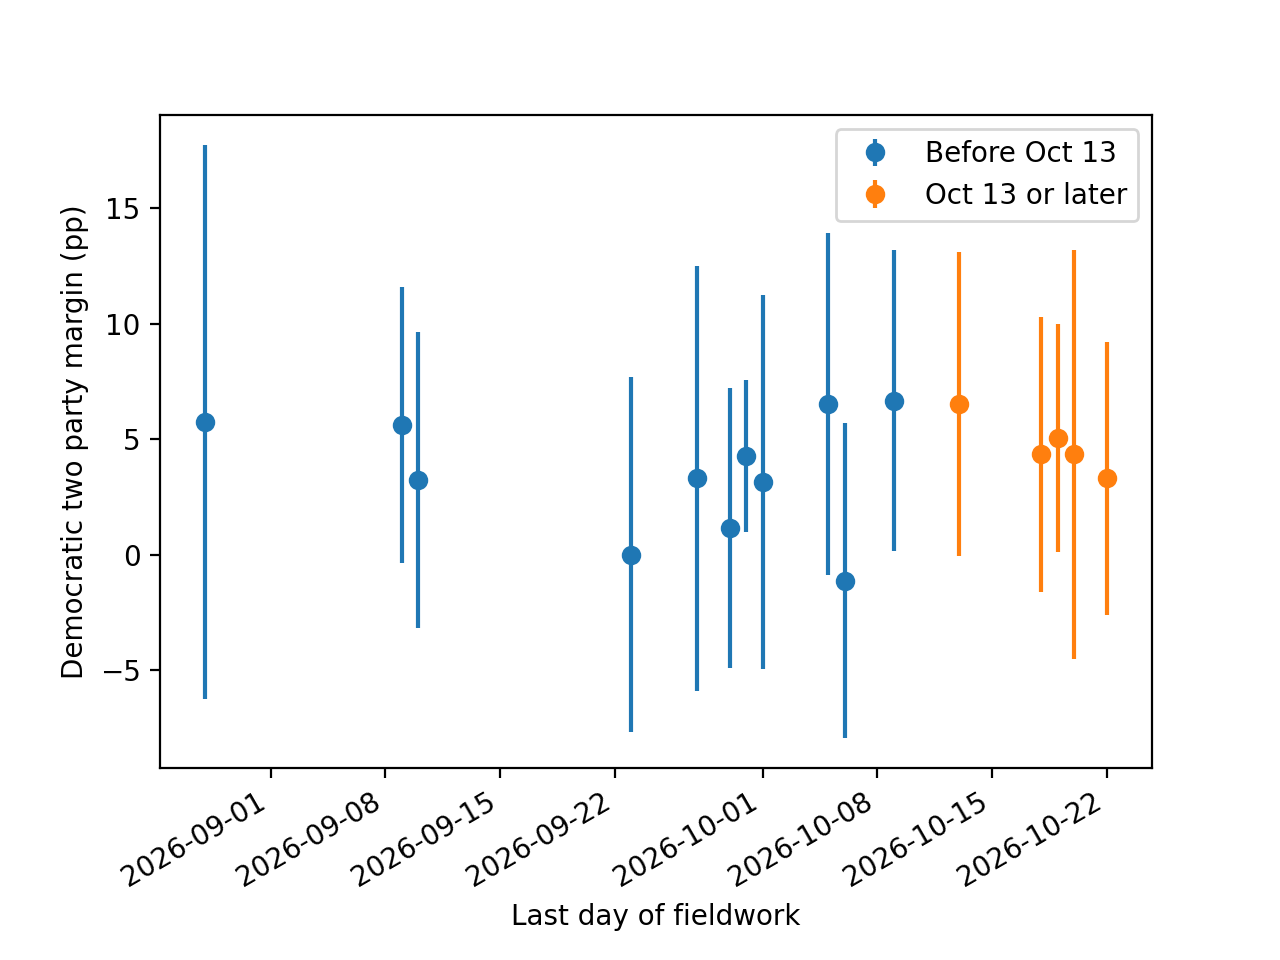
\includegraphics[width=\linewidth]{polls/poll_margins_over_time}
    \caption{Ohio Senate polls since August 2026: likely voters, nonpartisan sponsors, with 95\% sampling intervals. Orange: last field day on or after October 13.}
    \label{fig:polls}
  \end{minipage}\hfill
  \begin{minipage}[c]{0.40\textwidth}
    \centering
    \scriptsize
    \captionof{table}{Polls and historical Senate polling error, 2022 and 2024 (Democratic two party margin, pp)}
    \label{tab:polls}
    \textit{Ohio polls, last field day on or after Oct.\ 13}\par\smallskip
    \begin{tabular}{lr}
    \toprule
    Polls & 5 \\
    Respondents & 5{,}458 \\
    Mean & +4.7 \\
    Sample-weighted mean & +4.7 \\
    Median & +4.3 \\
    SD & 1.2 \\
    Min & +3.3 \\
    Max & +6.5 \\
    \bottomrule
    \end{tabular}
    \par\medskip
    \textit{Senate polling error (actual minus poll average)}\par\smallskip
    \begin{tabular}{lrrr}
    \toprule
     & Races & Mean & SD \\
    \midrule
    2022 & 19 & $-$2.3 & 5.8 \\
    2024 & 15 & $-$2.5 & 4.0 \\
    Pooled & 34 & $-$2.4 & 5.0 \\
    \bottomrule
    \end{tabular}
  \end{minipage}
\end{figure}

\subsection*{Demographics \& Incumbency}

Like a lot of rustbelt states, Ohio's electorate has sorted by education in the past decade and a half. Between 2012 and 2024 the Democratic presidential margin fell most in the counties with the fewest college graduates. This shift is already crudely reflected in Ohio's 2024 partisan lean, so the baseline needs no separate demographic adjustment.

\begin{figure}[H]
  \centering
  \begin{minipage}[t]{0.48\textwidth}
    \centering
    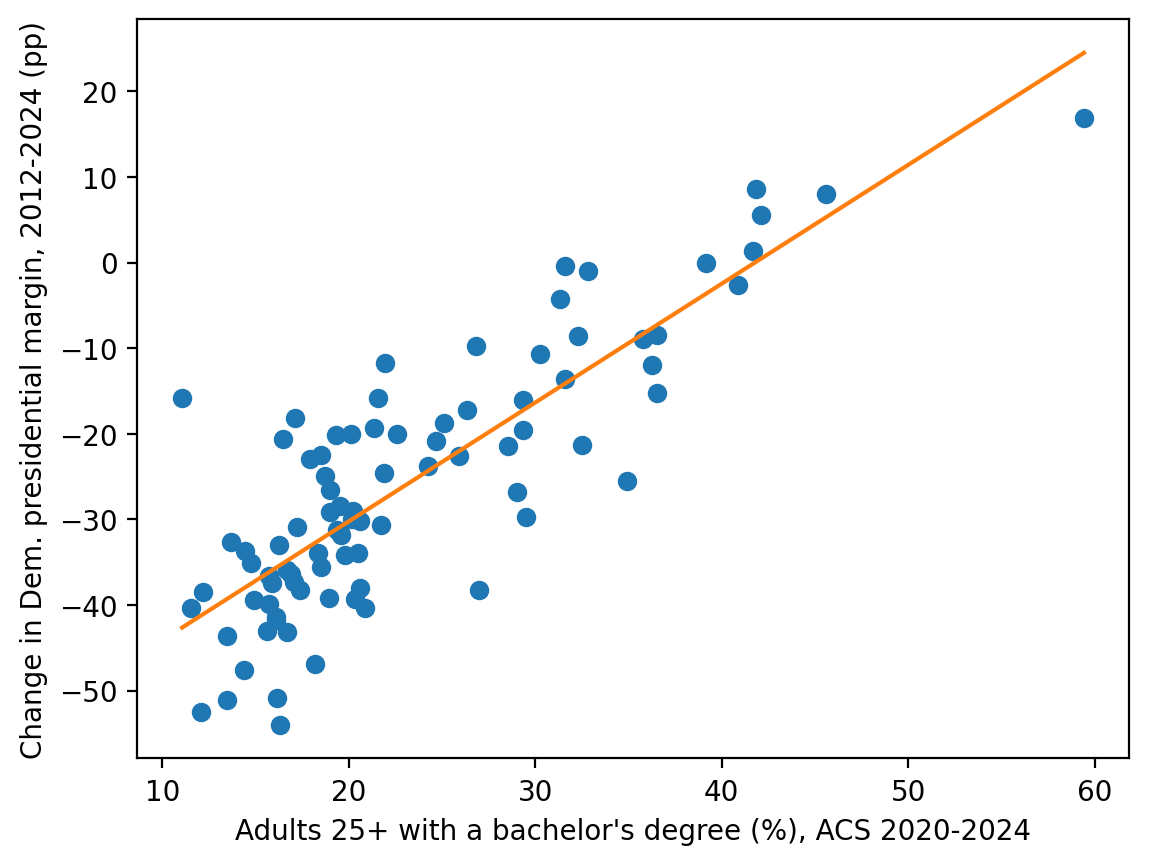
\includegraphics[width=\linewidth]{dem_incumbent/education_swing}
    \caption{Ohio counties: change in the Democratic presidential margin, 2012--2024, against college share.}
    \label{fig:edu_swing}
  \end{minipage}\hfill
  \begin{minipage}[t]{0.48\textwidth}
    \centering
    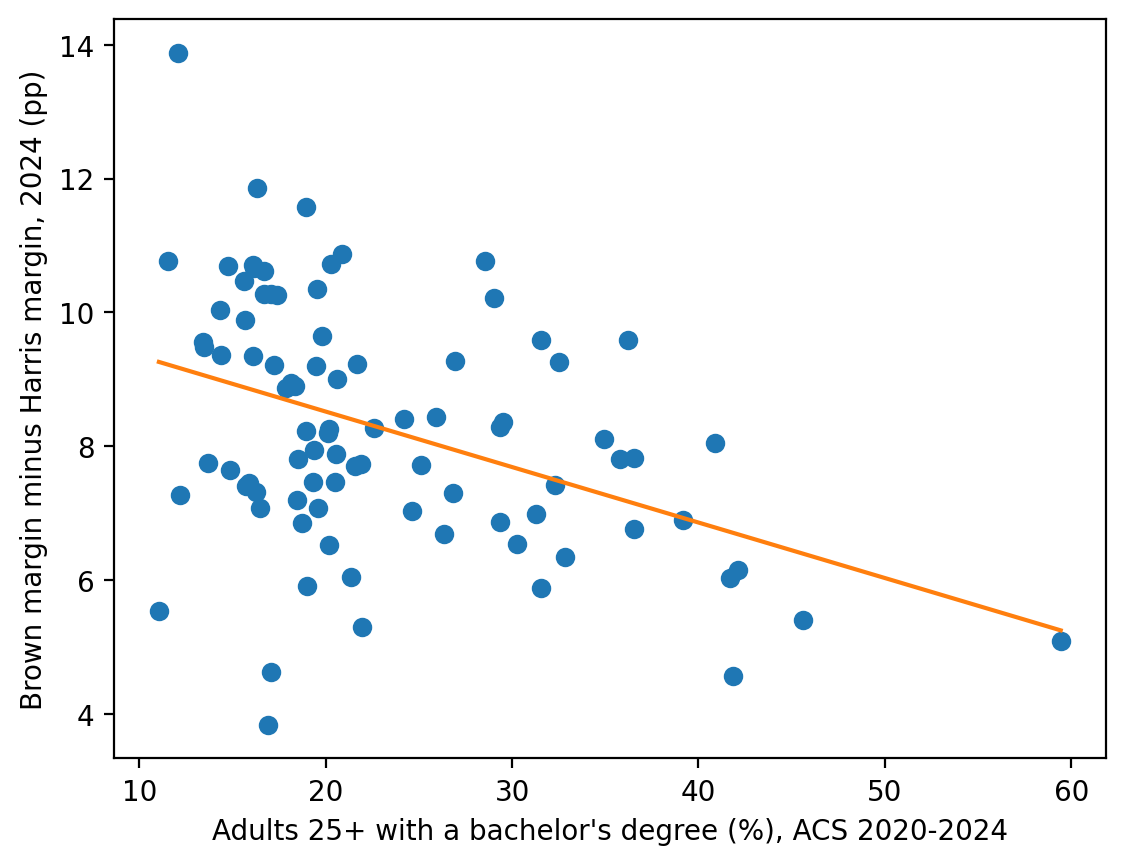
\includegraphics[width=\linewidth]{dem_incumbent/education_brown_runahead}
    \caption{Ohio counties: Brown's 2024 margin minus Harris's, against college share.}
    \label{fig:edu_brown}
  \end{minipage}
\end{figure}

Brown is essentially one of a few senate Democrat that goes against this trend, which explains his electoral success. In 2012 he ran ahead of Obama in over half of all counties, and in 2024 he ran ahead of Harris in every single county. Furthermore, he ran furthest ahead of the top of the ticket in the largest counties, but in 2024 he did so in the smallest, rural ones, and by more where fewer adults hold a college degree. 

\begin{figure}[H]
  \centering
  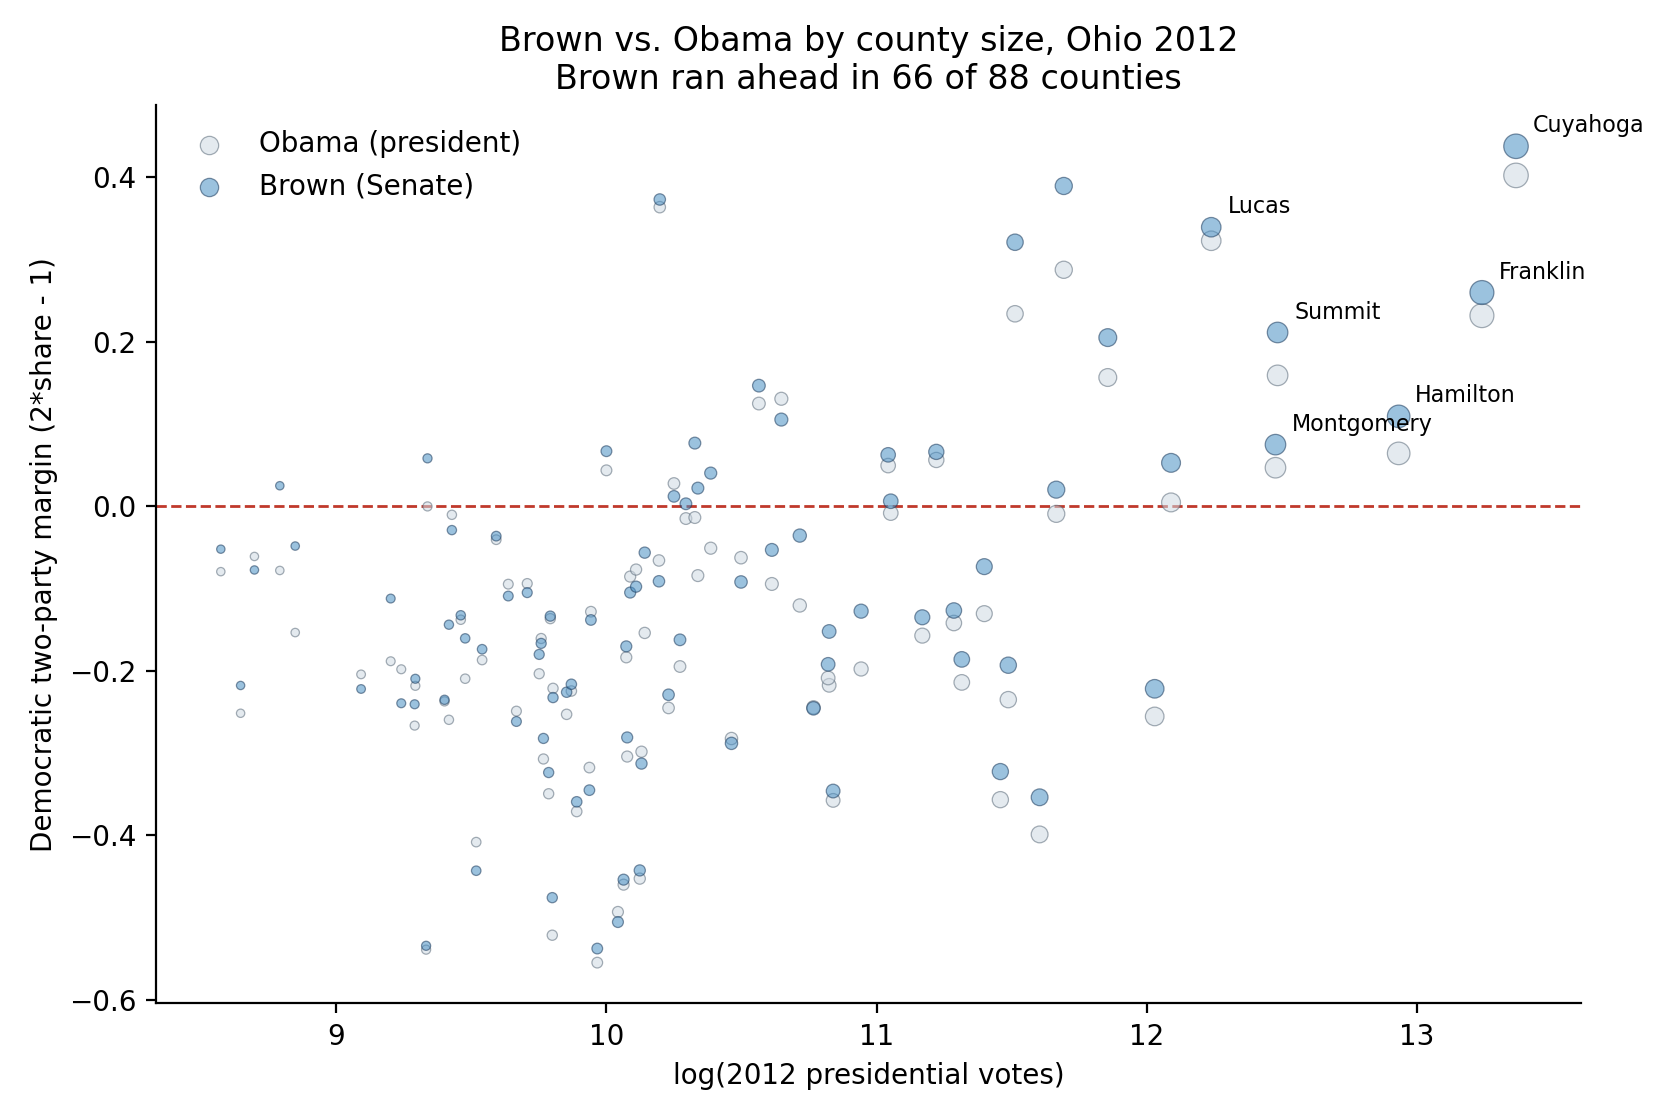
\includegraphics[width=0.48\textwidth]{dem_incumbent/brown_vs_obama_2012}\hfill
  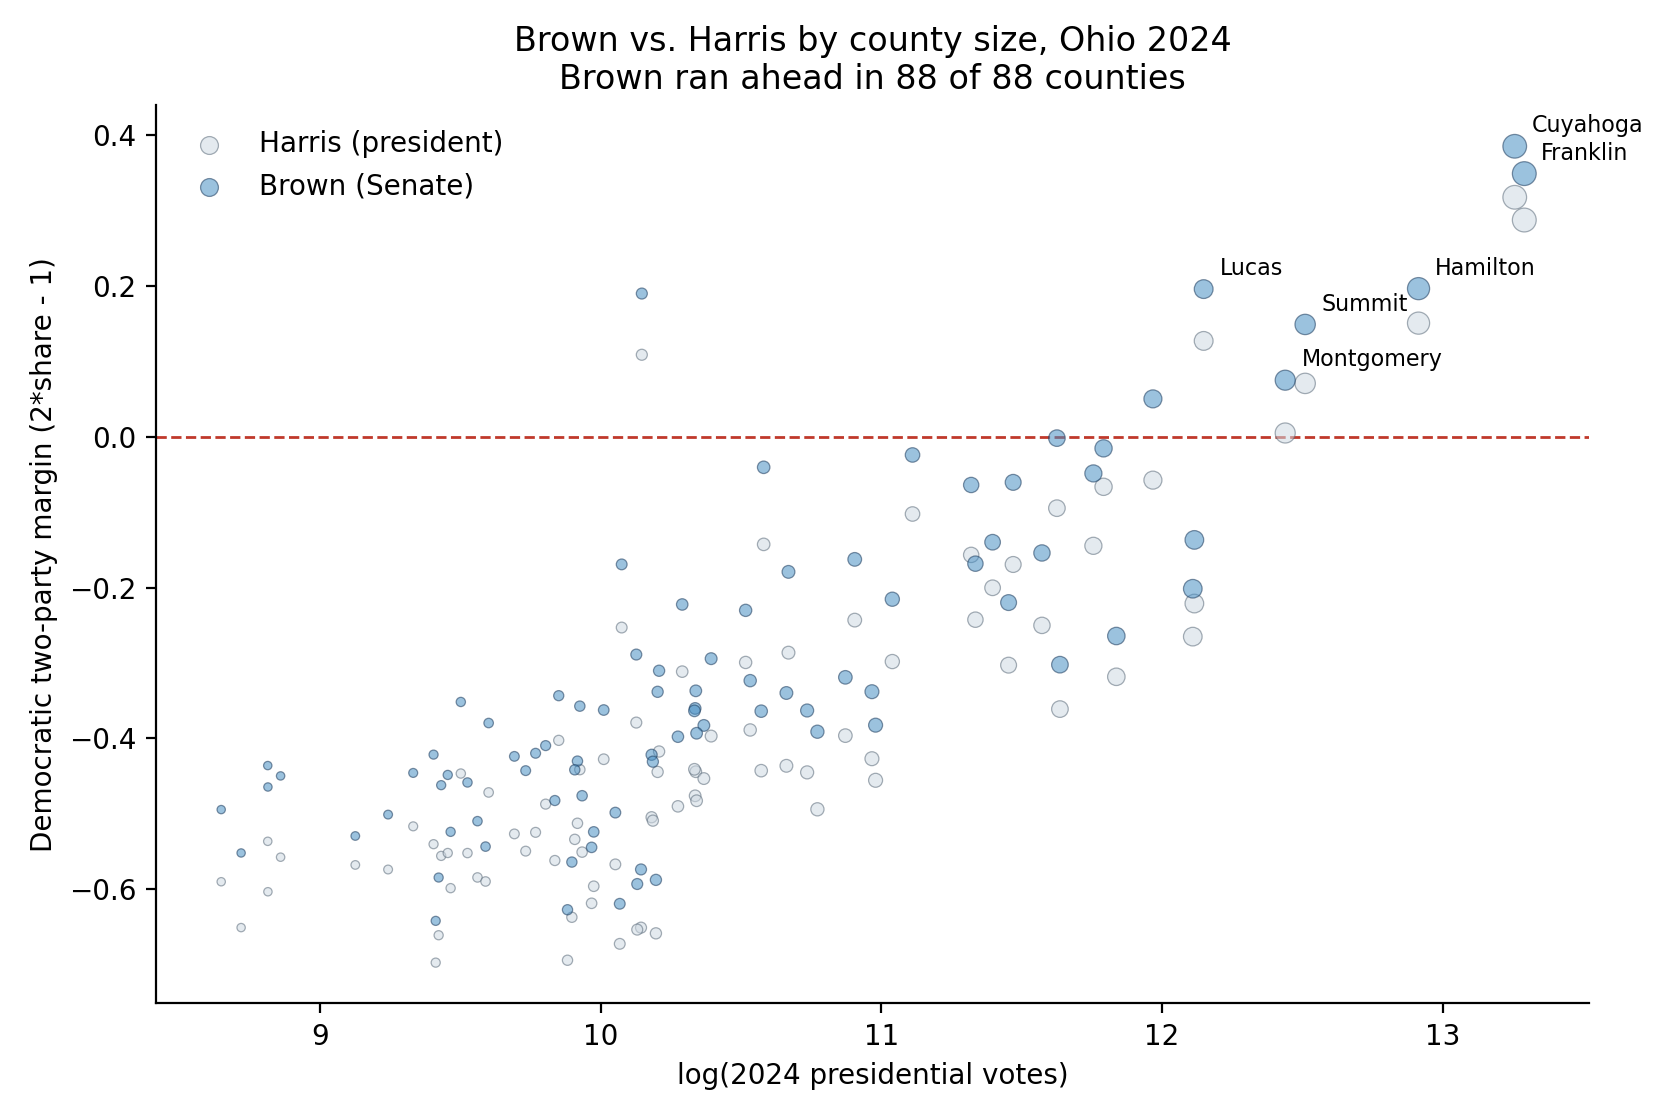
\includegraphics[width=0.48\textwidth]{dem_incumbent/brown_vs_harris_2024}
  \caption{Brown against the top of the ticket by county size: Obama in 2012 (left) and Harris in 2024 (right).}
  \label{fig:brown_pres}
\end{figure}

\begin{figure}[H]
  \centering
  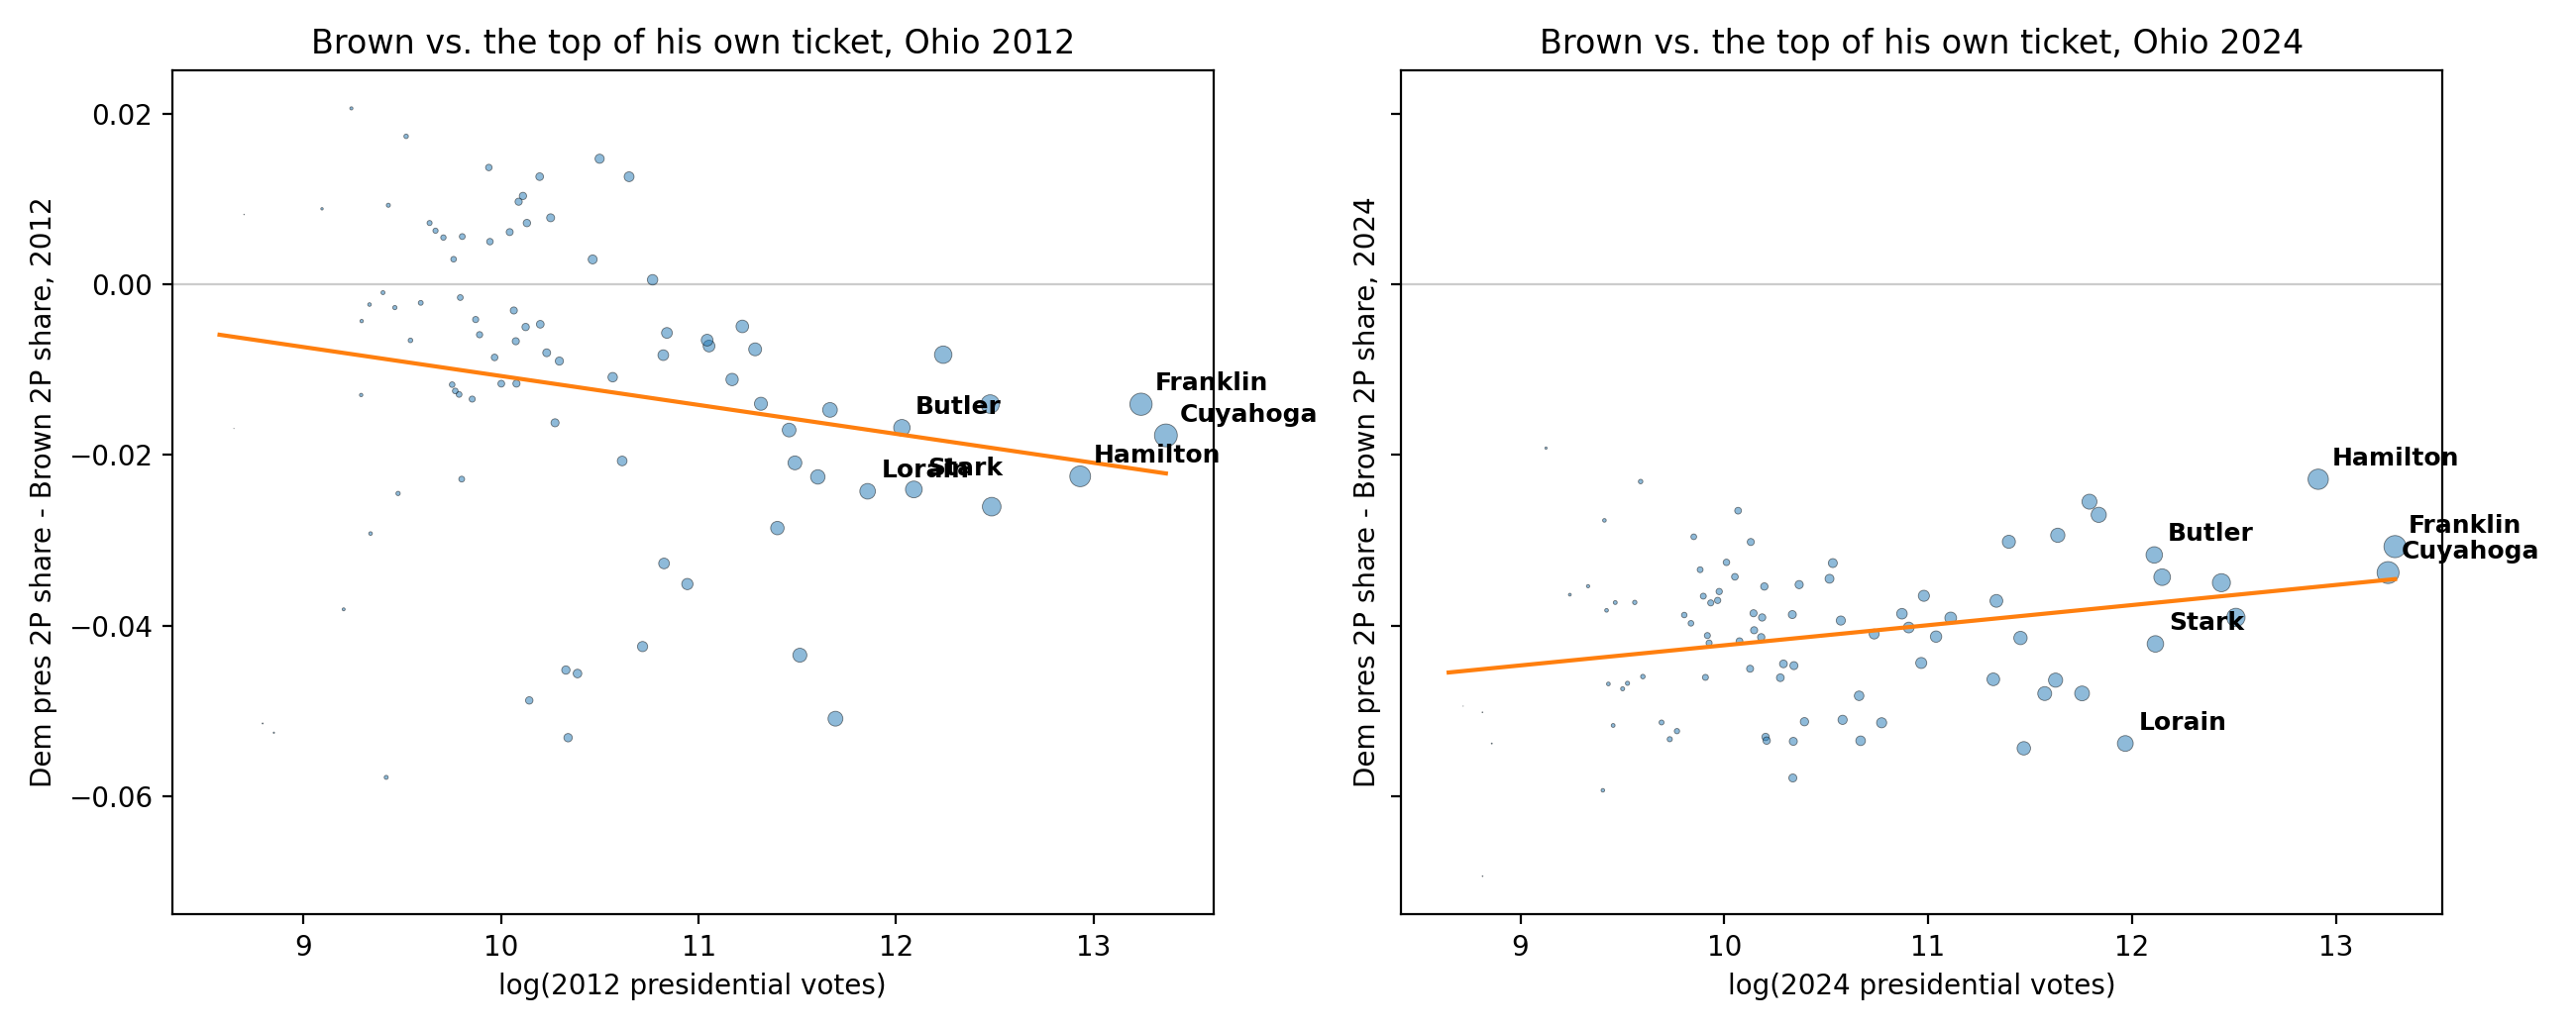
\includegraphics[width=0.9\textwidth]{dem_incumbent/brown_gap_by_county_size_2012_2024}
  \caption{Presidential share minus Brown's share by county size, 2012 and 2024 (negative: Brown ran ahead).}
  \label{fig:brown_gap}
\end{figure}

We choose not to treat either candidate as an incumbent. Husted was appointed rather than elected to the seat, and his last statewide race on his own (2014) says far less than Brown's 2024 result even though Brown lost that race. Instead, we group Brown's experience and appeal into one candidate adjustment. In 2024 Brown ran $5.3$ points of margin further ahead of Harris than the median Senate Democrat ran ahead of their party's presidential candidate (Figure~\ref{fig:runahead}). The baseline already credits $0.8$ points of this through the lagged Senate share, because that coefficient is estimated mostly from races in which the previous Senate candidate is not running again. Brown is, so we add the remaining $4.5$ points of margin ($2.2$ points of two party share) as the Brown appeal adjustment.

\begin{figure}[H]
  \centering
  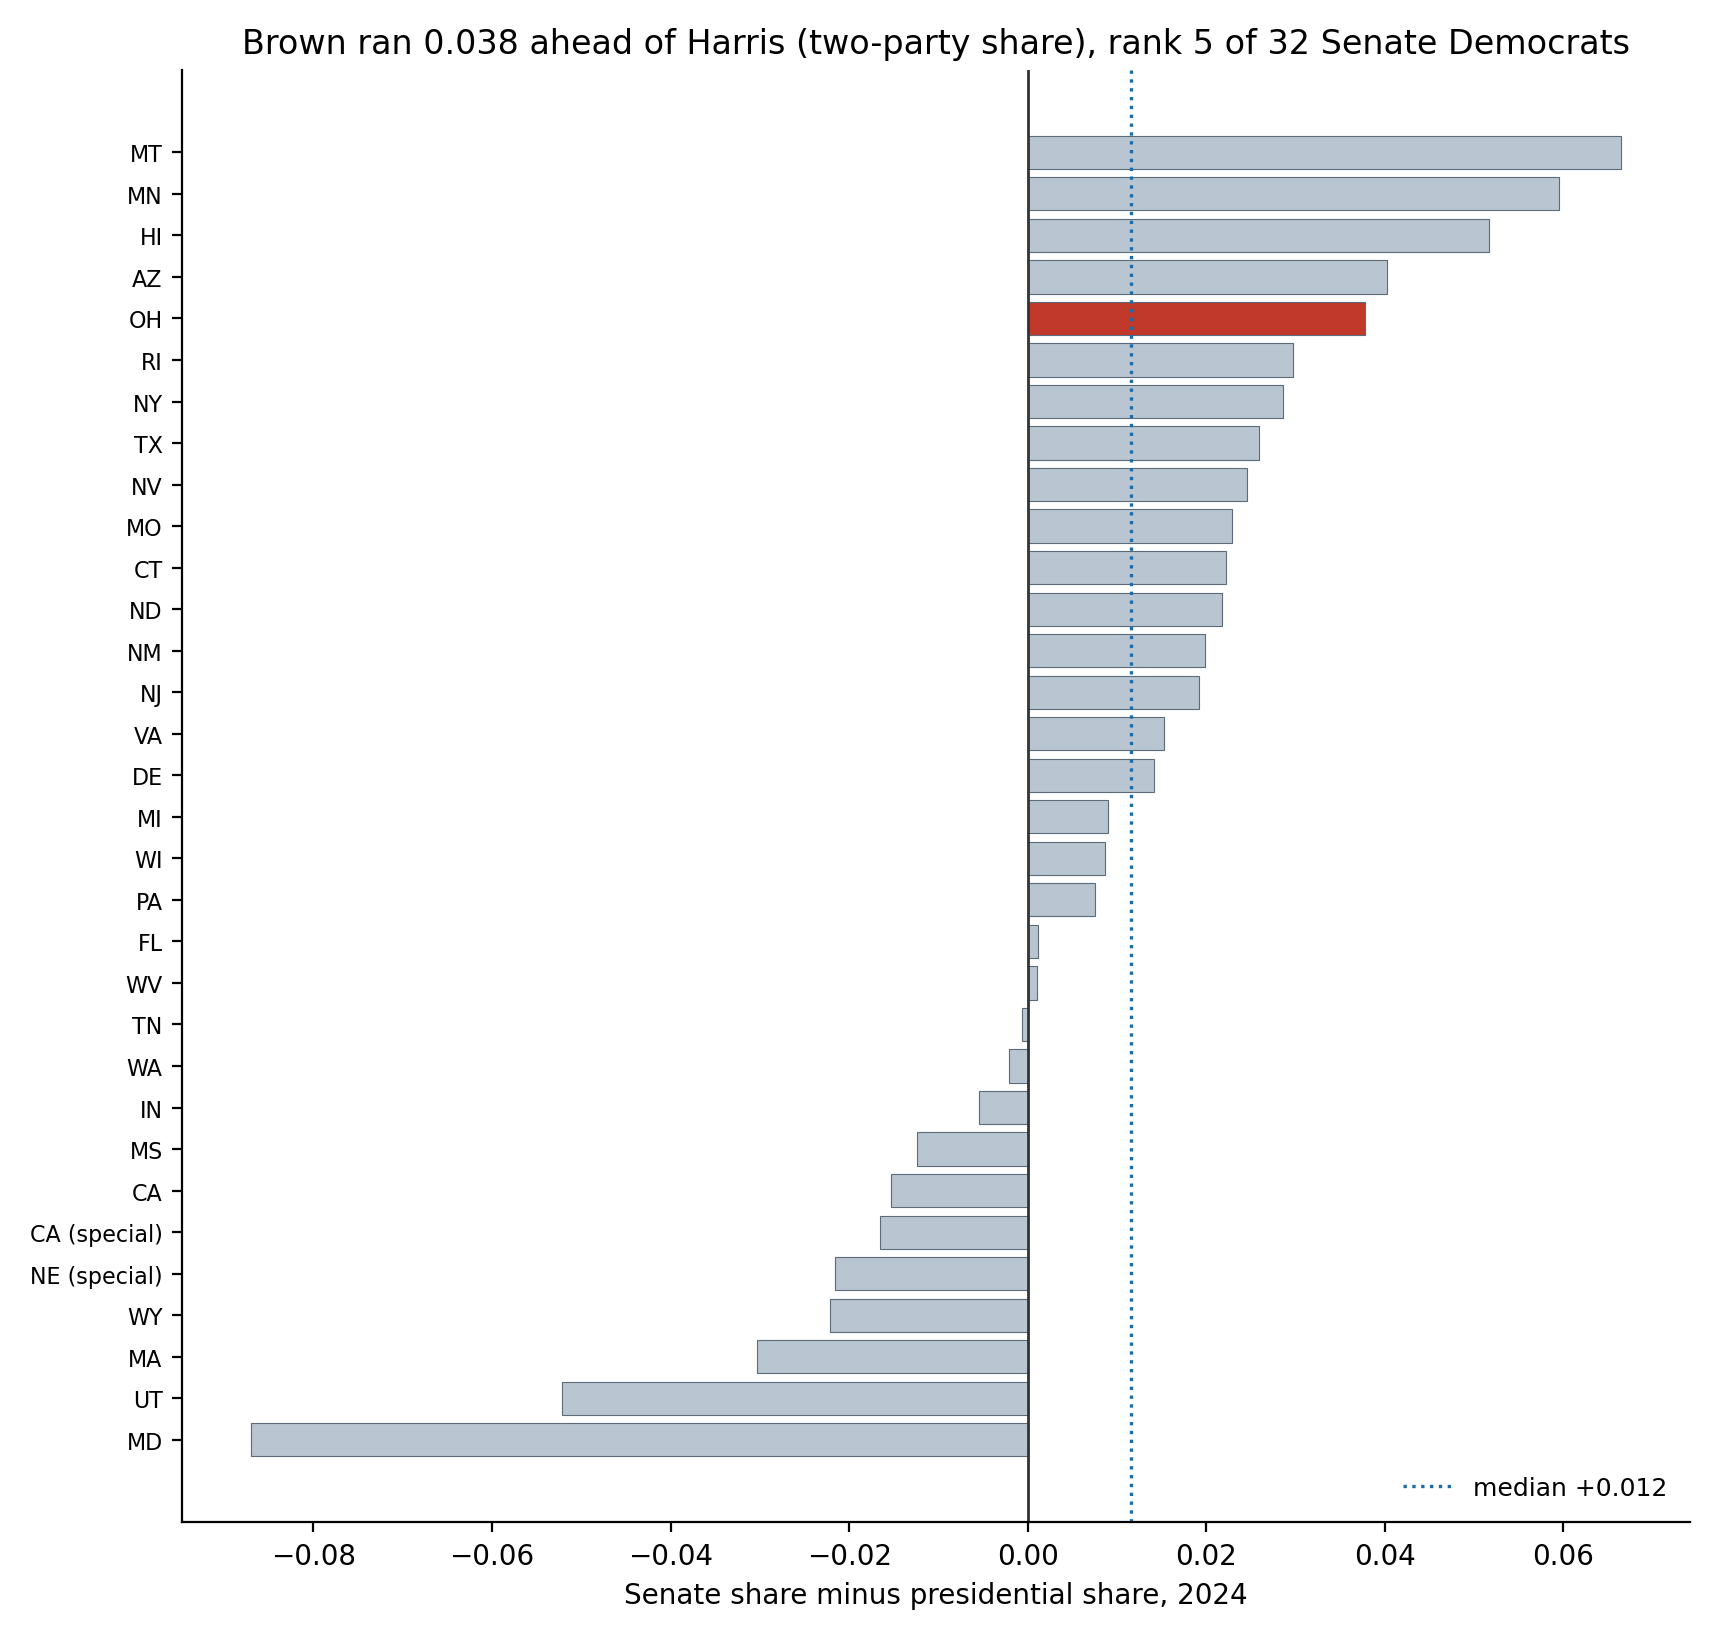
\includegraphics[width=0.6\textwidth]{dem_incumbent/runahead_2024_by_state}
  \caption{2024 Democratic Senate share minus presidential share, every 2024 Senate race (Ohio in red; dotted line: median).}
  \label{fig:runahead}
\end{figure}

\subsection*{Data}

Here's a table listing our sources for these past sections. For any incumbency codings or more particular pieces of quantiative or qualitative information e.g. specific two party shares in races we didn't plot the results or historical information, we just used the wikipedia and confirmed the cited source. 

\begin{table}[H]
  \centering
  \scriptsize
  \renewcommand{\arraystretch}{2}
  \caption{Data sources and cleaning choices}
  \label{tab:data}
  \begin{tabular}{>{\raggedright\arraybackslash}p{2.1cm} >{\raggedright\arraybackslash}p{4.2cm} >{\raggedright\arraybackslash}p{7.4cm}}
    \toprule
    Section & Source  \\
    \midrule
    Campaign finance & Federal Election Commission (FEC) quarterly reports of the principal campaign committees, January--September 2026  \\
    Demographics \& incumbency & U.S.\ Census Bureau, American Community Survey 5-year estimates (2006--10, 2020--24); MEDSL, OpenElections and Ohio Secretary of State county and precinct returns  \\
    Polling & Public releases of 32 Ohio polls, December 2025--October 2026; FiveThirtyEight Senate poll database (archived copy), 2022 and 2024  \\
    \bottomrule
  \end{tabular}
\end{table}

\newpage
\section*{Forecast Accounting \& Discussion}

Table~\ref{tab:coef} lists the coefficients of the baseline regression behind the forecast, and Figure~\ref{fig:waterfall} shows how each piece moves Brown's two party share. Ohio's partisan lean and the constant give $41.2\%$, the midterm under a Republican president adds $2.4$ points and Ohio's 2024 Senate share adds $7.0$, for a baseline of $50.6\%$ (margin $+1.2$). The Brown appeal adjustment raises this to $52.8\%$ (margin $+5.7$). Averaging this adjusted baseline equally with the poll-based estimate of $51.2\%$ (margin $+2.3$) gives our final forecast: Brown wins with $52.0\%$ of the two party vote, a margin of $+4.0$.

The forecast, conditional on trusting the underlying model, now just depends on whether or not Husted is an incumbent. Adding an incumbency term to the baseline (Table~\ref{tab:coef}, second row) gives Brown a margin of $-0.8$ when neither candidate is treated as an incumbent, but $-13.3$ when Husted is counted as one. Our forecast also assumes that Brown's 2024 appeal carries over in full against a stronger opponent, and that the polls' recent bias toward Democrats persists.

\begin{table}[H]
  \centering
  \footnotesize
  \caption{Baseline regression used in the forecast (Table~\ref{tab:baseline}, column 3), with and without an incumbency term $\text{Inc}_{s,t}$ ($+1$ Democratic incumbent, $-1$ Republican, $0$ open seat). Second row's 2026 margins: Husted not counted / counted as an incumbent.}
  \label{tab:coef}
  \begin{tabular}{lccccccccc}
    \toprule
     & Constant & $L_{s,\tau(t)}$ & $\text{MidD}_t$ & $\text{MidR}_t$ & $S_{s,\rho(t)}$ & $\text{Inc}_{s,t}$ & $R^2$ & Obs. & 2026 margin \\
    \midrule
    Baseline & 0.453 & 0.846 & $-$0.038 & 0.024 & 0.145 &  & 0.613 & 373 & +1.2 \\
    + incumbency & 0.498 & 0.657 & $-$0.041 & 0.008 & 0.046 & 0.063 & 0.734 & 373 & $-$0.8 / $-$13.3 \\
    \bottomrule
    \end{tabular}
\end{table}

\begin{figure}[H]
  \centering
  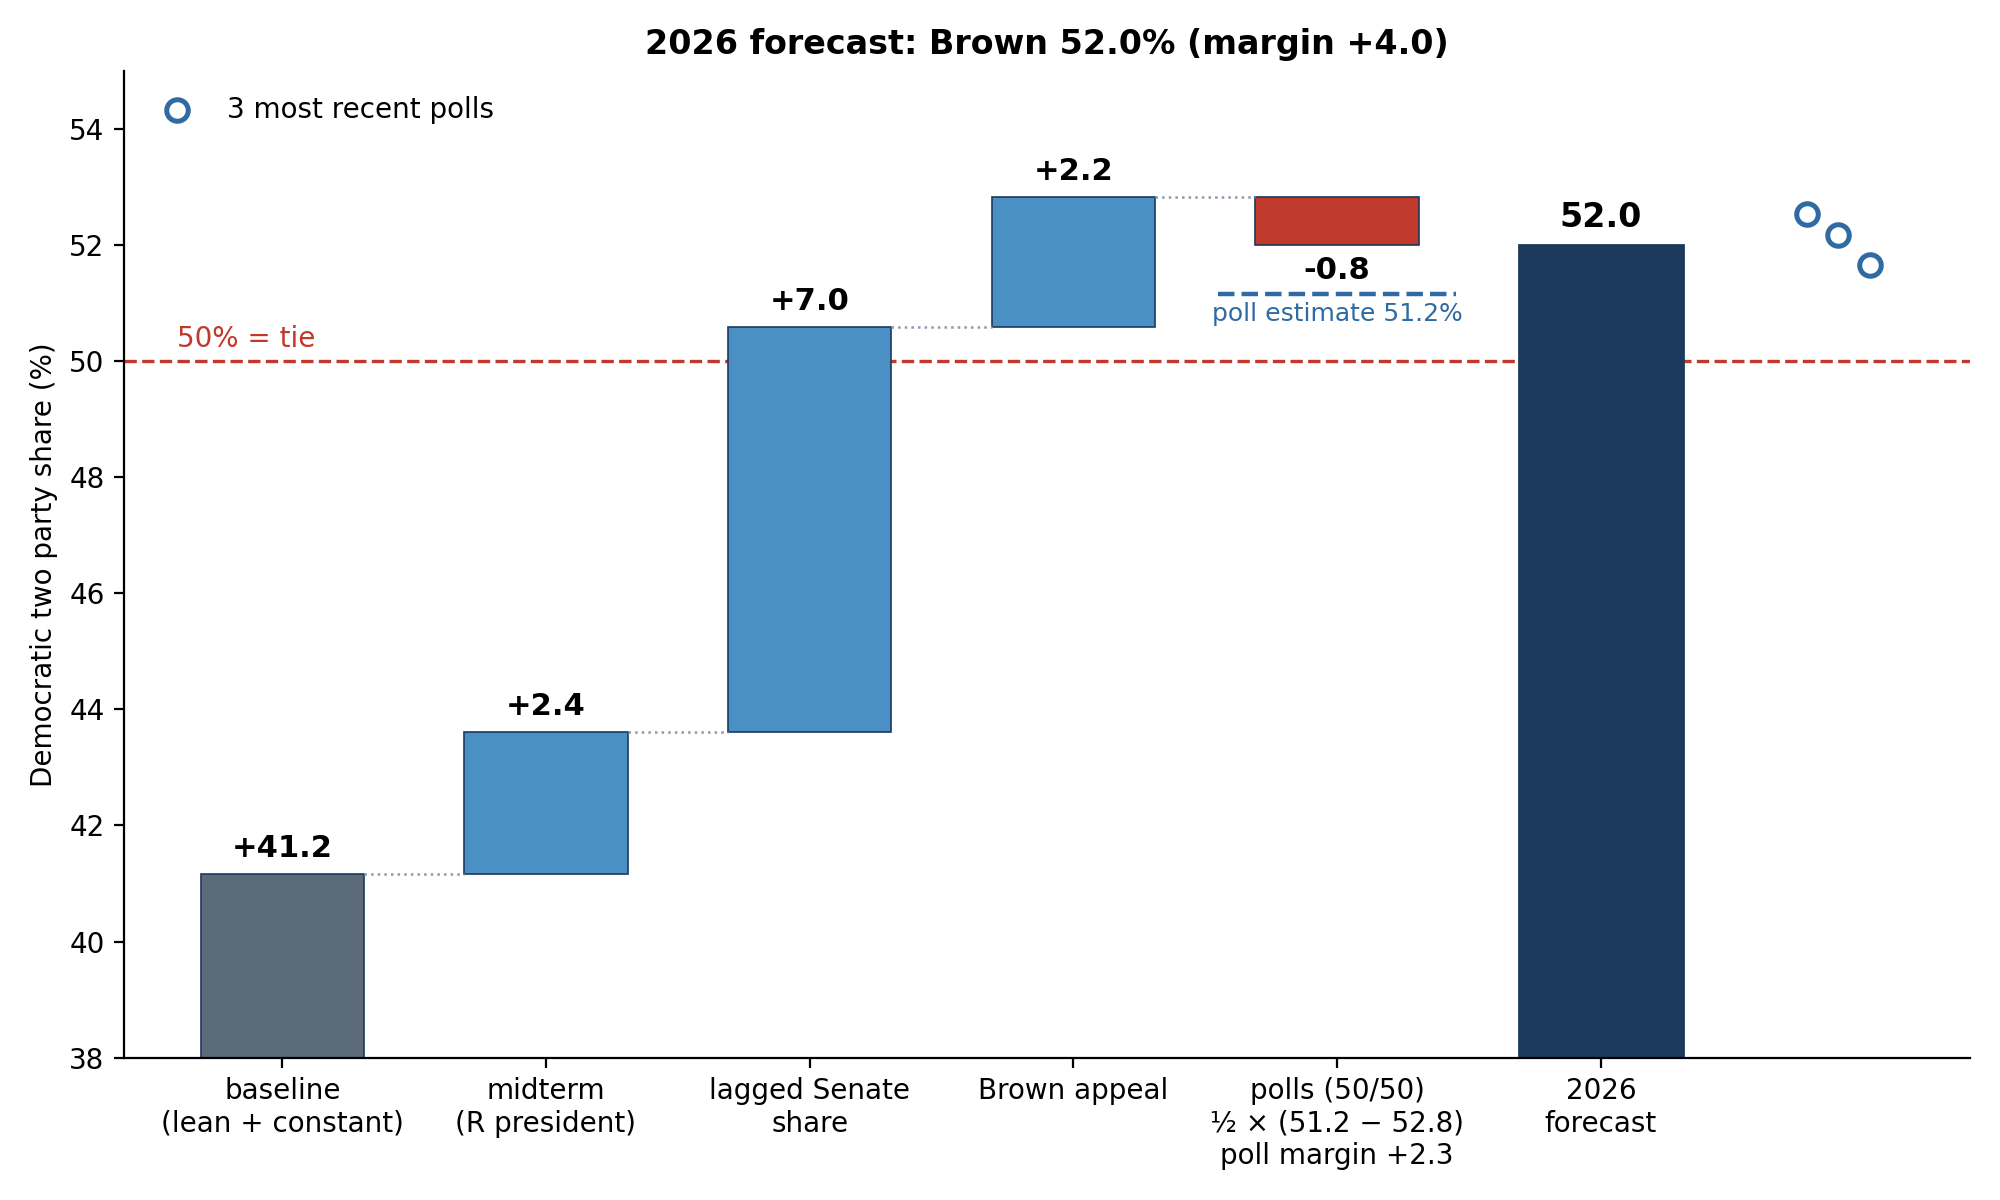
\includegraphics[width=0.85\textwidth]{forecast/forecast_waterfall}
  \caption{From the baseline to the 2026 forecast (Democratic two party share). The polls bar is half the gap between the poll-based estimate (51.2\%, margin $+2.3$) and the adjusted baseline (52.8\%).}
  \label{fig:waterfall}
\end{figure}







\end{document}